\begin{figure}

% \begin{subfigure}{0.5\textwidth}
% 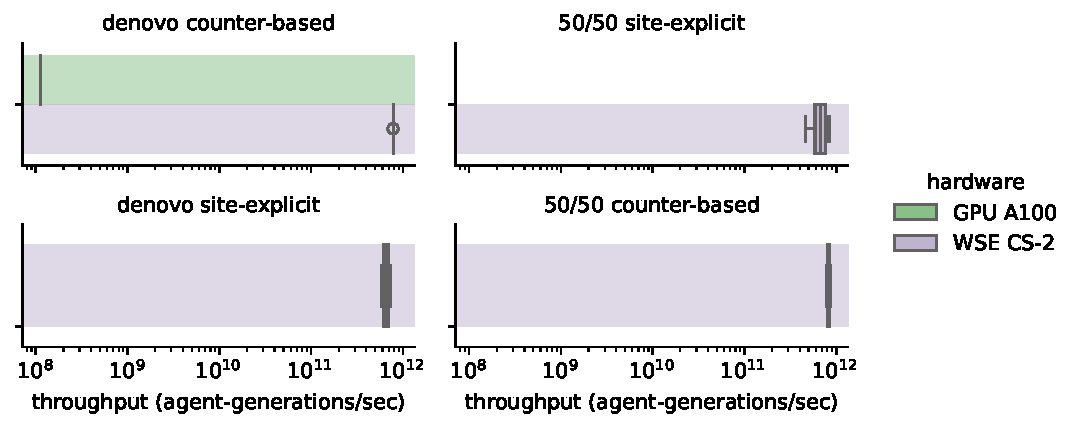
\includegraphics[width=\textwidth, trim={0cm 0cm 2.5cm 0cm}, clip]{binder/binder-perf-wse-vs-gpu.ipynb/binder/teeplots/col=experiment-design+hue=hardware+orient=h+viz=backplot+x=throughput-agent-generations-sec+ext=.pdf}
% \caption{throughput}
% \label{fig:perf:throughput}
% \end{subfigure}%
% \begin{subfigure}{0.49\textwidth}
\centering
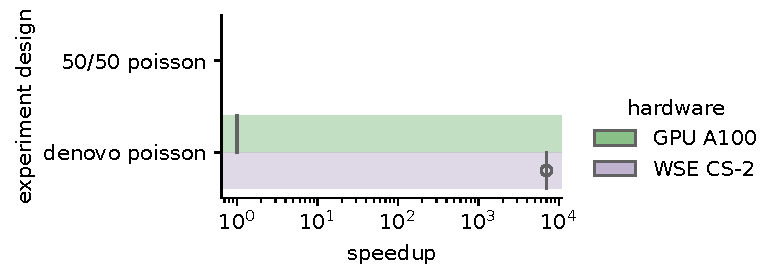
\includegraphics[width=0.85\linewidth]{binder/binder-perf-wse-vs-gpu.ipynb/binder/teeplots/hue=hardware+orient=h+viz=backplot+x=speedup+y=experiment-design+ext=.pdf}

\vspace{-2ex}
% ~
% \caption{speedup}
% \label{fig:perf:speedup}
% \end{subfigure}
\vspace{-2ex}

\caption{
  \textbf{Simulation performance on CPU, GPU, and WSE.}
  \footnotesize
  % CPU throughput was measured from NumPy-backed simulation code, GPU throughput was measured from equivalent CuPy-backed simulation code, and WSE throughput was measured from a comparable Cerebras Software Language implementation.
  % CPU experiments were single-core on AMD EPYC 7H12 (2.595 GHz), GPU hardware was NVIDIA A100, and WSE hardware was Cerebras CS-2.
  % Speedup was calculated relative to mean CPU throughput.
  % Shaded areas indicate bootstrapped 95\% confidence intervals with sample size $\geq 10$.
}
\label{fig:perf}

\vspace{-3ex}

\end{figure}
